\documentclass[11pt, a4paper]{article}

% Fonts and Encoding
\usepackage[utf8]{inputenc}
\usepackage[T1]{fontenc}

% Math and Symbols
\usepackage{amsmath, amssymb, amsthm, amsfonts, mathrsfs, mathtools}

% Layout and Geometry
\usepackage{geometry}
\geometry{a4paper, margin=1in}

% Formatting and Graphics
\usepackage{graphicx, xcolor, enumitem, booktabs, array, tabularx}

% TikZ for Illustrations
\usepackage{tikz}
\usetikzlibrary{arrows.meta, positioning, shapes.geometric, calc, backgrounds, matrix}

% Clickable Links and TOC
\usepackage{hyperref}
\hypersetup{
    colorlinks=true,
    linkcolor=blue,
    filecolor=magenta,      
    urlcolor=cyan,
    pdftitle={Comprehensive Guide to Inverse Laplace Transforms},
}

% Theorem Environments
\newtheorem{theorem}{Theorem}[section]
\newtheorem{lemma}[theorem]{Lemma}
\newtheorem{proposition}[theorem]{Proposition}
\newtheorem{corollary}[theorem]{Corollary}
\theoremstyle{definition}
\newtheorem{definition}{Definition}[section]
\newtheorem{axiom}{Axiom}[section]
\newtheorem{example}{Example}[section]
\theoremstyle{remark}
\newtheorem{remark}{Remark}[section]

% Custom Commands (Enforced standard notation)
\newcommand{\R}{\mathbb{R}}
\newcommand{\N}{\mathbb{N}}
\newcommand{\Z}{\mathbb{Z}}
\newcommand{\Q}{\mathbb{Q}}
\newcommand{\E}{\mathbb{E}}
\newcommand{\Prob}{\mathbb{P}}
\newcommand{\F}{\mathcal{F}}
\newcommand{\Laplace}{\mathcal{L}}
\newcommand{\InvLaplace}{\mathcal{L}^{-1}}

\title{\textbf{Comprehensive Guide to Inverse Laplace Transforms}}
\author{Tashfeen Omran}
\date{\today}

\begin{document}

\maketitle
\tableofcontents
\newpage

\section{Part 1: Comprehensive Introduction, Context, and Prerequisites}

\subsection{Core Concepts}
The Laplace Transform is an integral transform that converts a function of a real variable $t$ (often time) into a function of a complex variable $s$ (complex frequency). The \textbf{Inverse Laplace Transform}, denoted as $\InvLaplace\{F(s)\}$, is the operation that reverses this process, taking a function from the frequency domain back to the time domain. 

Mathematically, if $\Laplace\{f(t)\} = F(s)$, then $f(t) = \InvLaplace\{F(s)\}$. While the forward transform is defined by an explicit integral ($\int_0^\infty f(t)e^{-st} \, dt$), the inverse transform is formally defined by the complex Bromwich integral. However, in practice, we almost never use the complex integral. Instead, we rely on algebraic manipulation (like partial fraction decomposition and completing the square) to massage $F(s)$ into recognizable forms that match a standard table of known transforms.

\subsection{Intuition and Derivation}
Think of the Laplace transform as a mathematical prism. Just as a prism splits white light into its component colors (frequencies), the Laplace transform splits a complex differential equation into its algebraic frequency components. In the $s$-domain, calculus operations (differentiation and integration) become basic arithmetic (multiplication and division by $s$). 

The Inverse Laplace Transform is the process of reassembling those frequencies back into the original signal. We solve the easy algebraic puzzle in the $s$-domain, and then use the inverse transform to translate the solution back into the real world ($t$-domain).

\subsection{Historical Context and Motivation}
In the late 19th century, the English electrical engineer Oliver Heaviside developed a controversial "operational calculus" to solve differential equations related to electrical circuits. He treated the derivative operator as an algebraic variable. Mathematicians initially rejected his methods because they lacked rigorous proof, despite yielding correct answers. Later, mathematicians realized that Heaviside's operational calculus was perfectly justified by the integral transforms previously studied by Pierre-Simon Laplace in the 1780s. The Laplace transform was thus formalized as the rigorous foundation for solving linear ordinary differential equations (ODEs) without needing to guess solutions or find integrating factors.

\subsection{Key Formulas}
The foundation of finding inverse transforms is the lookup table. The most critical pairs are:
\begin{itemize}
    \item $\InvLaplace\left\{ \frac{1}{s} \right\} = 1$
    \item $\InvLaplace\left\{ \frac{n!}{s^{n+1}} \right\} = t^n$
    \item $\InvLaplace\left\{ \frac{1}{s-a} \right\} = e^{at}$
    \item $\InvLaplace\left\{ \frac{b}{s^2 + b^2} \right\} = \sin(bt)$
    \item $\InvLaplace\left\{ \frac{s}{s^2 + b^2} \right\} = \cos(bt)$
\end{itemize}
Additionally, the \textbf{First Translation (Shifting) Theorem} states that $\InvLaplace\{F(s-a)\} = e^{at}f(t)$.

\subsection{Prerequisites}
To succeed in this topic, you must have absolute mastery over:
\begin{enumerate}
    \item \textbf{Partial Fraction Decomposition:} Breaking down complex rational functions into simpler fractions. You must know how to handle distinct linear roots, repeated linear roots, and irreducible quadratic roots.
    \item \textbf{Completing the Square:} Essential for dealing with irreducible quadratics in the denominator to match them with shifted sine and cosine transforms.
    \item \textbf{Algebraic Manipulation:} Factoring, expanding, and splitting numerators (e.g., $\frac{s+5}{s^2+1} = \frac{s}{s^2+1} + \frac{5}{s^2+1}$).
\end{enumerate}

\vspace{1em}
\begin{center}
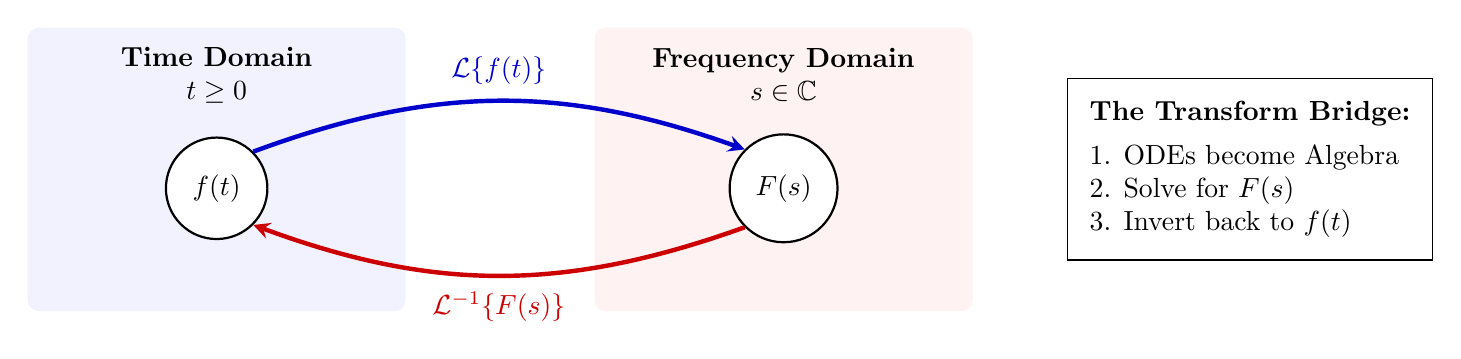
\begin{tikzpicture}[scale=1.2]
    % Backgrounds
    \fill[blue!5!white, rounded corners] (-2.5, -1.5) rectangle (1.5, 1.5);
    \fill[red!5!white, rounded corners] (3.5, -1.5) rectangle (7.5, 1.5);
    
    % Nodes
    \node[align=center] at (-0.5, 1) {\textbf{Time Domain} \\ $t \ge 0$};
    \node[align=center] at (5.5, 1) {\textbf{Frequency Domain} \\ $s \in \mathbb{C}$};
    
    \node[draw, thick, fill=white, circle, inner sep=6pt] (ft) at (-0.5, -0.2) {$f(t)$};
    \node[draw, thick, fill=white, circle, inner sep=6pt] (Fs) at (5.5, -0.2) {$F(s)$};
    
    % Arrows
    \draw[->, ultra thick, blue!80!black, >=stealth] (ft.north east) to[bend left=20] node[above=2pt] {$\Laplace\{f(t)\}$} (Fs.north west);
    \draw[->, ultra thick, red!80!black, >=stealth] (Fs.south west) to[bend left=20] node[below=2pt] {$\InvLaplace\{F(s)\}$} (ft.south east);
    
    % Legend
    \node[align=left, anchor=west, inner sep=8pt, draw, fill=white] at (8.5, 0) {
        \textbf{The Transform Bridge:} \\[4pt]
        1. ODEs become Algebra \\
        2. Solve for $F(s)$ \\
        3. Invert back to $f(t)$
    };
\end{tikzpicture}
\end{center}

\newpage
\section{Part 2: Detailed Homework Solutions}

\subsection*{Problem 1}
\textbf{Determine the inverse Laplace transform of the function below:}
\[ F(s) = \frac{9}{s^2 + 81} \]

\textbf{Solution:}
We recognize the form of the sine transform: $\Laplace\{\sin(bt)\} = \frac{b}{s^2 + b^2}$.
Here, $b^2 = 81$, which implies $b = 9$. The numerator is exactly $b$.
\[ \InvLaplace\left\{ \frac{9}{s^2 + 9^2} \right\} = \sin(9t) \]
\textbf{Final Answer:} $\sin(9t)$

\subsection*{Problem 2}
\textbf{Determine the inverse Laplace transform of the function below:}
\[ F(s) = \frac{14}{s^2 + 9} \]

\textbf{Solution:}
This is similar to the sine transform, where $b^2 = 9 \implies b = 3$. However, the numerator is 14, not 3. We use the linearity of the inverse transform to adjust the constant:
\begin{align*}
    \InvLaplace\left\{ \frac{14}{s^2 + 9} \right\} &= 14 \cdot \InvLaplace\left\{ \frac{1}{s^2 + 9} \right\} \\
    &= \frac{14}{3} \cdot \InvLaplace\left\{ \frac{3}{s^2 + 3^2} \right\} \\
    &= \frac{14}{3} \sin(3t)
\end{align*}
\textbf{Final Answer:} $\frac{14}{3} \sin(3t)$

\subsection*{Problem 3}
\textbf{Determine the inverse Laplace transform of the function below:}
\[ F(s) = \frac{4s + 22}{s^2 + 8s + 25} \]

\textbf{Solution:}
The denominator is an irreducible quadratic. We must complete the square:
\[ s^2 + 8s + 25 = (s^2 + 8s + 16) + 9 = (s+4)^2 + 3^2 \]
Now, rewrite the numerator to match the shifted term $(s+4)$:
\[ 4s + 22 = 4(s+4) - 16 + 22 = 4(s+4) + 6 \]
Substitute this back into the transform:
\begin{align*}
    F(s) &= \frac{4(s+4) + 6}{(s+4)^2 + 3^2} \\
    &= 4 \left( \frac{s+4}{(s+4)^2 + 3^2} \right) + 2 \left( \frac{3}{(s+4)^2 + 3^2} \right)
\end{align*}
Using the First Translation Theorem ($\Laplace\{e^{at}f(t)\} = F(s-a)$):
\[ f(t) = 4e^{-4t}\cos(3t) + 2e^{-4t}\sin(3t) \]
\textbf{Final Answer:} $e^{-4t}(4\cos(3t) + 2\sin(3t))$

\subsection*{Problem 4}
\textbf{Determine the inverse Laplace transform of the function below:}
\[ F(s) = \frac{1}{s^7} \]

\textbf{Solution:}
We use the power rule: $\Laplace\{t^n\} = \frac{n!}{s^{n+1}}$.
Here, $n+1 = 7 \implies n = 6$. We need $6!$ in the numerator.
\begin{align*}
    \InvLaplace\left\{ \frac{1}{s^7} \right\} &= \frac{1}{6!} \InvLaplace\left\{ \frac{6!}{s^7} \right\} \\
    &= \frac{1}{720} t^6
\end{align*}
\textbf{Final Answer:} $\frac{t^6}{720}$

\subsection*{Problem 5}
\textbf{Determine the inverse Laplace transform of the function below:}
\[ F(s) = \frac{s - 8}{4s^2 + s + 8} \]

\textbf{Solution:}
First, factor out the leading coefficient of the denominator to make completing the square easier:
\[ 4s^2 + s + 8 = 4\left(s^2 + \frac{1}{4}s + 2\right) \]
Complete the square for $s^2 + \frac{1}{4}s + 2$:
\[ s^2 + \frac{1}{4}s + 2 = \left(s + \frac{1}{8}\right)^2 - \frac{1}{64} + 2 = \left(s + \frac{1}{8}\right)^2 + \frac{127}{64} \]
Now, rewrite the numerator in terms of $(s + 1/8)$:
\[ s - 8 = \left(s + \frac{1}{8}\right) - \frac{1}{8} - 8 = \left(s + \frac{1}{8}\right) - \frac{65}{8} \]
Substitute everything back into $F(s)$:
\begin{align*}
    F(s) &= \frac{1}{4} \frac{\left(s + \frac{1}{8}\right) - \frac{65}{8}}{\left(s + \frac{1}{8}\right)^2 + \frac{127}{64}} \\
    &= \frac{1}{4} \frac{s + \frac{1}{8}}{\left(s + \frac{1}{8}\right)^2 + \frac{127}{64}} - \frac{65}{32} \frac{1}{\left(s + \frac{1}{8}\right)^2 + \frac{127}{64}}
\end{align*}
Let $\omega^2 = \frac{127}{64} \implies \omega = \frac{\sqrt{127}}{8}$. We need $\omega$ in the numerator of the second term:
\begin{align*}
    F(s) &= \frac{1}{4} \frac{s + \frac{1}{8}}{\left(s + \frac{1}{8}\right)^2 + \omega^2} - \frac{65}{32} \cdot \frac{1}{\omega} \cdot \frac{\omega}{\left(s + \frac{1}{8}\right)^2 + \omega^2} \\
    &= \frac{1}{4} \frac{s + \frac{1}{8}}{\left(s + \frac{1}{8}\right)^2 + \omega^2} - \frac{65}{32} \left(\frac{8}{\sqrt{127}}\right) \frac{\omega}{\left(s + \frac{1}{8}\right)^2 + \omega^2} \\
    &= \frac{1}{4} \frac{s + \frac{1}{8}}{\left(s + \frac{1}{8}\right)^2 + \omega^2} - \frac{65}{4\sqrt{127}} \frac{\omega}{\left(s + \frac{1}{8}\right)^2 + \omega^2}
\end{align*}
Taking the inverse transform:
\[ f(t) = \frac{1}{4} e^{-t/8} \cos\left(\frac{\sqrt{127}}{8}t\right) - \frac{65}{4\sqrt{127}} e^{-t/8} \sin\left(\frac{\sqrt{127}}{8}t\right) \]
\textbf{Final Answer:} $\frac{1}{4} e^{-t/8} \cos\left(\frac{\sqrt{127}}{8}t\right) - \frac{65}{4\sqrt{127}} e^{-t/8} \sin\left(\frac{\sqrt{127}}{8}t\right)$

\subsection*{Problem 6}
\textbf{Determine the partial fraction expansion for the rational function below:}
\[ F(s) = \frac{13s + 64}{(s+3)(s^2+16)} \]

\textbf{Solution:}
Set up the partial fraction decomposition. Since $s^2+16$ is an irreducible quadratic, it requires a linear numerator:
\[ \frac{13s + 64}{(s+3)(s^2+16)} = \frac{A}{s+3} + \frac{Bs+C}{s^2+16} \]
Multiply by the common denominator:
\[ 13s + 64 = A(s^2+16) + (Bs+C)(s+3) \]
To find $A$, let $s = -3$:
\[ 13(-3) + 64 = A((-3)^2 + 16) \implies -39 + 64 = 25A \implies 25 = 25A \implies A = 1 \]
Now expand the right side to find $B$ and $C$:
\[ 13s + 64 = 1(s^2+16) + Bs^2 + 3Bs + Cs + 3C \]
\[ 13s + 64 = (1+B)s^2 + (3B+C)s + (16+3C) \]
Equate coefficients:
\begin{align*}
    s^2 \text{ terms:} \quad & 0 = 1 + B \implies B = -1 \\
    s^0 \text{ terms:} \quad & 64 = 16 + 3C \implies 48 = 3C \implies C = 16
\end{align*}
Substitute $A, B, C$ back into the expansion:
\[ F(s) = \frac{1}{s+3} + \frac{-s+16}{s^2+16} \]
\textbf{Final Answer:} $\frac{1}{s+3} + \frac{-s+16}{s^2+16}$

\subsection*{Problem 7}
\textbf{Determine $\InvLaplace\{F\}$ for:}
\[ F(s) = \frac{8s^2 - 13s + 6}{s(s-4)(s-2)} \]

\textbf{Solution:}
Set up the partial fraction decomposition for distinct linear roots:
\[ \frac{8s^2 - 13s + 6}{s(s-4)(s-2)} = \frac{A}{s} + \frac{B}{s-4} + \frac{C}{s-2} \]
We use the Heaviside Cover-Up Method:
\begin{align*}
    A &= \left. \frac{8s^2 - 13s + 6}{(s-4)(s-2)} \right|_{s=0} = \frac{6}{(-4)(-2)} = \frac{6}{8} = \frac{3}{4} \\[6pt]
    B &= \left. \frac{8s^2 - 13s + 6}{s(s-2)} \right|_{s=4} = \frac{8(16) - 13(4) + 6}{4(2)} = \frac{128 - 52 + 6}{8} = \frac{82}{8} = \frac{41}{4} \\[6pt]
    C &= \left. \frac{8s^2 - 13s + 6}{s(s-4)} \right|_{s=2} = \frac{8(4) - 13(2) + 6}{2(-2)} = \frac{32 - 26 + 6}{-4} = \frac{12}{-4} = -3
\end{align*}
Thus, the function is:
\[ F(s) = \frac{3/4}{s} + \frac{41/4}{s-4} - \frac{3}{s-2} \]
Taking the inverse transform:
\[ f(t) = \frac{3}{4} + \frac{41}{4}e^{4t} - 3e^{2t} \]
\textbf{Final Answer:} $\frac{3}{4} + \frac{41}{4}e^{4t} - 3e^{2t}$

\subsection*{Problem 8}
\textbf{Determine $\InvLaplace\{F\}$ for:}
\[ F(s) = \frac{3s^2 + 31s + 84}{(s+5)^2(s+6)} \]

\textbf{Solution:}
Set up the partial fraction decomposition for a repeated linear root:
\[ \frac{3s^2 + 31s + 84}{(s+5)^2(s+6)} = \frac{A}{s+5} + \frac{B}{(s+5)^2} + \frac{C}{s+6} \]
Multiply by the denominator:
\[ 3s^2 + 31s + 84 = A(s+5)(s+6) + B(s+6) + C(s+5)^2 \]
Let $s = -5$:
\[ 3(25) - 31(5) + 84 = B(1) \implies 75 - 155 + 84 = B \implies B = 4 \]
Let $s = -6$:
\[ 3(36) - 31(6) + 84 = C(-1)^2 \implies 108 - 186 + 84 = C \implies C = 6 \]
To find $A$, compare the $s^2$ coefficients on both sides:
\[ 3 = A + C \implies 3 = A + 6 \implies A = -3 \]
The expansion is:
\[ F(s) = \frac{-3}{s+5} + \frac{4}{(s+5)^2} + \frac{6}{s+6} \]
Taking the inverse transform (using $\InvLaplace\{\frac{1}{(s-a)^2}\} = te^{at}$):
\[ f(t) = -3e^{-5t} + 4te^{-5t} + 6e^{-6t} \]
\textbf{Final Answer:} $-3e^{-5t} + 4te^{-5t} + 6e^{-6t}$

\subsection*{Problem 9}
\textbf{Determine $\InvLaplace\{F\}$ for:}
\[ s^2 F(s) + 2s F(s) - 15 F(s) = \frac{2s^2 + 3}{s^2 + 4s} \]

\textbf{Solution:}
First, factor the left side and isolate $F(s)$:
\[ F(s)(s^2 + 2s - 15) = \frac{2s^2 + 3}{s(s + 4)} \]
\[ F(s)(s+5)(s-3) = \frac{2s^2 + 3}{s(s + 4)} \]
\[ F(s) = \frac{2s^2 + 3}{s(s+4)(s+5)(s-3)} \]
Set up partial fractions:
\[ \frac{2s^2 + 3}{s(s+4)(s+5)(s-3)} = \frac{A}{s} + \frac{B}{s+4} + \frac{C}{s+5} + \frac{D}{s-3} \]
Using the Heaviside Cover-Up Method:
\begin{align*}
    A &= \left. \frac{2s^2 + 3}{(s+4)(s+5)(s-3)} \right|_{s=0} = \frac{3}{(4)(5)(-3)} = -\frac{1}{20} \\[6pt]
    B &= \left. \frac{2s^2 + 3}{s(s+5)(s-3)} \right|_{s=-4} = \frac{2(16) + 3}{(-4)(1)(-7)} = \frac{35}{28} = \frac{5}{4} \\[6pt]
    C &= \left. \frac{2s^2 + 3}{s(s+4)(s-3)} \right|_{s=-5} = \frac{2(25) + 3}{(-5)(-1)(-8)} = \frac{53}{-40} = -\frac{53}{40} \\[6pt]
    D &= \left. \frac{2s^2 + 3}{s(s+4)(s+5)} \right|_{s=3} = \frac{2(9) + 3}{(3)(7)(8)} = \frac{21}{168} = \frac{1}{8}
\end{align*}
The expansion is:
\[ F(s) = -\frac{1/20}{s} + \frac{5/4}{s+4} - \frac{53/40}{s+5} + \frac{1/8}{s-3} \]
Taking the inverse transform:
\[ f(t) = -\frac{1}{20} + \frac{5}{4}e^{-4t} - \frac{53}{40}e^{-5t} + \frac{1}{8}e^{3t} \]
\textbf{Final Answer:} $-\frac{1}{20} + \frac{5}{4}e^{-4t} - \frac{53}{40}e^{-5t} + \frac{1}{8}e^{3t}$

\subsection*{Problem 10}
\textbf{Determine $\InvLaplace\{F\}$ for:}
\[ s F(s) - 5 F(s) = \frac{4s + 1}{s^2 + 10s + 25} \]

\textbf{Solution:}
Factor the left side and the denominator on the right side:
\[ F(s)(s - 5) = \frac{4s + 1}{(s+5)^2} \]
\[ F(s) = \frac{4s + 1}{(s-5)(s+5)^2} \]
Set up partial fractions:
\[ \frac{4s + 1}{(s-5)(s+5)^2} = \frac{A}{s-5} + \frac{B}{s+5} + \frac{C}{(s+5)^2} \]
Multiply by the denominator:
\[ 4s + 1 = A(s+5)^2 + B(s-5)(s+5) + C(s-5) \]
Let $s = 5$:
\[ 4(5) + 1 = A(10)^2 \implies 21 = 100A \implies A = \frac{21}{100} \]
Let $s = -5$:
\[ 4(-5) + 1 = C(-10) \implies -19 = -10C \implies C = \frac{19}{10} \]
To find $B$, compare the $s^2$ coefficients:
\[ 0 = A + B \implies B = -A = -\frac{21}{100} \]
The expansion is:
\[ F(s) = \frac{21/100}{s-5} - \frac{21/100}{s+5} + \frac{19/10}{(s+5)^2} \]
Taking the inverse transform:
\[ f(t) = \frac{21}{100}e^{5t} - \frac{21}{100}e^{-5t} + \frac{19}{10}te^{-5t} \]
\textbf{Final Answer:} $\frac{21}{100}e^{5t} - \frac{21}{100}e^{-5t} + \frac{19}{10}te^{-5t}$

\subsection*{Problem 11}
\textbf{Determine $\InvLaplace\{F\}$ for:}
\[ F(s) = \frac{7s^2 + 72s + 137}{(s-3)(s^2 + 6s + 25)} \]

\textbf{Solution:}
Set up partial fractions (note the irreducible quadratic):
\[ \frac{7s^2 + 72s + 137}{(s-3)(s^2 + 6s + 25)} = \frac{A}{s-3} + \frac{Bs+C}{s^2 + 6s + 25} \]
Multiply by the denominator:
\[ 7s^2 + 72s + 137 = A(s^2 + 6s + 25) + (Bs+C)(s-3) \]
Let $s = 3$:
\[ 7(9) + 72(3) + 137 = A(9 + 18 + 25) \implies 63 + 216 + 137 = 52A \implies 416 = 52A \implies A = 8 \]
Compare $s^2$ coefficients:
\[ 7 = A + B \implies 7 = 8 + B \implies B = -1 \]
Compare constant terms ($s^0$):
\[ 137 = 25A - 3C \implies 137 = 25(8) - 3C \implies 137 = 200 - 3C \implies 3C = 63 \implies C = 21 \]
So the expansion is:
\[ F(s) = \frac{8}{s-3} + \frac{-s+21}{s^2 + 6s + 25} \]
Complete the square for the quadratic: $s^2 + 6s + 25 = (s+3)^2 + 16$.
Rewrite the numerator $-s+21$ in terms of $(s+3)$:
\[ -s + 21 = -(s+3) + 3 + 21 = -(s+3) + 24 \]
Substitute back:
\begin{align*}
    F(s) &= \frac{8}{s-3} + \frac{-(s+3) + 24}{(s+3)^2 + 4^2} \\
    &= \frac{8}{s-3} - \frac{s+3}{(s+3)^2 + 4^2} + 6 \left( \frac{4}{(s+3)^2 + 4^2} \right)
\end{align*}
Taking the inverse transform:
\[ f(t) = 8e^{3t} - e^{-3t}\cos(4t) + 6e^{-3t}\sin(4t) \]
\textbf{Final Answer:} $8e^{3t} - e^{-3t}\cos(4t) + 6e^{-3t}\sin(4t)$

\subsection*{Problem 12}
\textbf{Determine $\InvLaplace\{F\}$ for:}
\[ F(s) = \frac{8s^3 - 54s^2 - 3s + 27}{s^3(s-9)} \]

\textbf{Solution:}
Set up partial fractions for the repeated root $s^3$:
\[ \frac{8s^3 - 54s^2 - 3s + 27}{s^3(s-9)} = \frac{A}{s} + \frac{B}{s^2} + \frac{C}{s^3} + \frac{D}{s-9} \]
Multiply by the denominator:
\[ 8s^3 - 54s^2 - 3s + 27 = As^2(s-9) + Bs(s-9) + C(s-9) + Ds^3 \]
Let $s = 0$:
\[ 27 = C(-9) \implies C = -3 \]
Let $s = 9$:
\[ 8(729) - 54(81) - 3(9) + 27 = D(729) \implies 5832 - 4374 - 27 + 27 = 729D \implies 1458 = 729D \implies D = 2 \]
Compare $s^3$ coefficients:
\[ 8 = A + D \implies 8 = A + 2 \implies A = 6 \]
To find $B$, compare $s^2$ coefficients:
\[ -54 = -9A + B \implies -54 = -9(6) + B \implies -54 = -54 + B \implies B = 0 \]
The expansion is:
\[ F(s) = \frac{6}{s} - \frac{3}{s^3} + \frac{2}{s-9} \]
Rewrite the $s^3$ term to match the transform table $\frac{n!}{s^{n+1}}$ where $n=2$:
\[ F(s) = \frac{6}{s} - \frac{3}{2} \left( \frac{2!}{s^3} \right) + \frac{2}{s-9} \]
Taking the inverse transform:
\[ f(t) = 6 - \frac{3}{2}t^2 + 2e^{9t} \]
\textbf{Final Answer:} $6 - \frac{3}{2}t^2 + 2e^{9t}$

\newpage
\section{Part 3: In-Depth Analysis of Problems and Techniques}

\subsection{A) Problem Types and General Approach}
The homework assignment can be categorized into three distinct problem types:

\begin{enumerate}
    \item \textbf{Direct Table Lookups (Problems 1, 2, 4):}
    \begin{itemize}
        \item \textit{Strategy:} These require no major algebraic restructuring. The goal is simply to multiply and divide by a constant to perfectly match the numerator required by the standard Laplace table (e.g., ensuring $n!$ is in the numerator for $t^n$, or $b$ is in the numerator for $\sin(bt)$).
    \end{itemize}
    \item \textbf{Completing the Square (Problems 3, 5):}
    \begin{itemize}
        \item \textit{Strategy:} When the denominator is an irreducible quadratic ($b^2 - 4ac < 0$), you must complete the square to form $(s-a)^2 + \omega^2$. Then, algebraically force the numerator to contain the exact term $(s-a)$. This allows you to split the fraction into a shifted cosine and a shifted sine term.
    \end{itemize}
    \item \textbf{Partial Fraction Decomposition (Problems 6, 7, 8, 9, 10, 11, 12):}
    \begin{itemize}
        \item \textit{Strategy:} These problems feature complex rational functions. The strategy is to factor the denominator completely, set up the correct partial fraction template (distinct linear, repeated linear, or irreducible quadratic), solve for the unknown constants, and then invert each simple fraction individually.
    \end{itemize}
\end{enumerate}

\subsection{B) Key Algebraic and Calculus Manipulations}
\begin{itemize}
    \item \textbf{The Heaviside Cover-Up Method:} Used extensively in Problems 7 and 9. When dealing with distinct linear factors like $\frac{P(s)}{(s-a)(s-b)}$, you can find the coefficient for $\frac{A}{s-a}$ by "covering up" $(s-a)$ in the original fraction and evaluating the rest at $s=a$. This bypasses solving massive systems of equations.
    \item \textbf{Numerator Shifting (The "Add and Subtract" Trick):} Seen in Problems 3, 5, and 11. After completing the square in the denominator to get $(s-a)^2$, the numerator usually looks like $Cs + D$. You must rewrite $s$ as $(s-a) + a$ to split the fraction properly. For example, in Problem 11, $-s + 21$ was rewritten as $-(s+3) + 3 + 21 = -(s+3) + 24$.
    \item \textbf{Coefficient Matching:} Used in Problems 6, 8, 10, 11, and 12. When the Cover-Up method fails (due to repeated roots or irreducible quadratics), we expand the equation and equate the coefficients of $s^n$ on both sides to create a solvable linear system.
    \item \textbf{Factoring out Leading Coefficients:} In Problem 5, the denominator was $4s^2 + s + 8$. Attempting to complete the square with a leading $4$ is a common source of errors. The crucial trick was factoring out the $4$ first: $4(s^2 + \frac{1}{4}s + 2)$, completing the square inside the parentheses, and leaving the $\frac{1}{4}$ as a global multiplier.
\end{itemize}

\newpage
\section{Part 4: "Cheatsheet" and Tips for Success}

\subsection{Essential Laplace Transform Table}
\renewcommand{\arraystretch}{1.5}
\begin{table}[h!]
\centering
\begin{tabularx}{\textwidth}{>{\raggedright\arraybackslash}X >{$\displaystyle}c<{$} >{$\displaystyle}c<{$}}
\toprule
\textbf{Function Name} & \textbf{Time Domain } f(t) & \textbf{Frequency Domain } F(s) \\
\midrule
Constant & 1 & \frac{1}{s} \\
\addlinespace[4pt]
Polynomial & t^n & \frac{n!}{s^{n+1}} \\
\addlinespace[4pt]
Exponential & e^{at} & \frac{1}{s-a} \\
\addlinespace[4pt]
Sine & \sin(bt) & \frac{b}{s^2+b^2} \\
\addlinespace[4pt]
Cosine & \cos(bt) & \frac{s}{s^2+b^2} \\
\addlinespace[4pt]
Shifted Polynomial & t^n e^{at} & \frac{n!}{(s-a)^{n+1}} \\
\addlinespace[4pt]
Shifted Sine & e^{at}\sin(bt) & \frac{b}{(s-a)^2+b^2} \\
\addlinespace[4pt]
Shifted Cosine & e^{at}\cos(bt) & \frac{s-a}{(s-a)^2+b^2} \\
\bottomrule
\end{tabularx}
\end{table}

\subsection{Pro-Tips and Shortcuts}
\begin{itemize}
    \item \textbf{The $s \to \infty$ Sanity Check:} For any strictly proper rational function $F(s)$, $\lim_{s \to \infty} sF(s) = f(0)$ (Initial Value Theorem). Furthermore, the sum of the coefficients in a partial fraction expansion of a strictly proper fraction where the denominator degree is at least 2 higher than the numerator must equal zero. (e.g., in Problem 9, $-\frac{1}{20} + \frac{5}{4} - \frac{53}{40} + \frac{1}{8} = 0$).
    \item \textbf{Repeated Roots Shortcut:} For $F(s) = \frac{P(s)}{(s-a)^n}$, you can find the coefficients by evaluating derivatives. $C_k = \frac{1}{k!} \frac{d^k}{ds^k} [ (s-a)^n F(s) ]_{s=a}$.
\end{itemize}

\subsection{Common Pitfalls to Avoid}
\begin{itemize}
    \item \textbf{Forgetting the Factorial:} When inverting $\frac{1}{s^4}$, students often write $\frac{t^3}{4}$ or $t^3$. You MUST multiply and divide by $3! = 6$. The correct answer is $\frac{t^3}{6}$.
    \item \textbf{Sign Errors in Exponentials:} The transform of $e^{at}$ is $\frac{1}{s-a}$. Therefore, $\frac{1}{s+5}$ corresponds to $e^{-5t}$, not $e^{5t}$. Always flip the sign!
    \item \textbf{Misidentifying Irreducible Quadratics:} Before completing the square, quickly check the discriminant $b^2 - 4ac$. If it is positive, the quadratic can be factored into real linear roots, and you should use partial fractions instead of completing the square.
\end{itemize}

\newpage
\section{Part 5: Conceptual Synthesis and The "Big Picture"}

\subsection{A) Thematic Connections}
The central theme of the Laplace Transform is \textbf{Isomorphism}—a mapping that preserves mathematical structure while changing the domain to make operations easier. We have seen this theme before:
\begin{itemize}
    \item \textbf{Logarithms:} In algebra, logarithms map multiplication into addition ($\log(ab) = \log a + \log b$). If you want to multiply massive numbers, you take their logs, add them, and take the inverse log.
    \item \textbf{Diagonalization:} In linear algebra, changing the basis of a matrix to its eigenvectors turns matrix exponentiation (a very hard problem) into scalar exponentiation along a diagonal (a very easy problem).
\end{itemize}
The Laplace transform does exactly this for calculus. It maps the derivative operator $\frac{d}{dt}$ to the algebraic multiplication operator $s$. It turns the hard problem of solving differential equations into the easy problem of solving algebraic fractions.

\subsection{B) Forward and Backward Links}
\textbf{Backward Links:} This topic relies heavily on Calculus II integration techniques (specifically improper integrals for the forward transform) and Pre-Calculus algebra (partial fractions and completing the square). 

\textbf{Forward Links:} Mastering the Inverse Laplace Transform is the absolute bedrock for:
\begin{itemize}
    \item \textbf{Control Theory:} In engineering, systems are modeled as "Transfer Functions" $H(s) = \frac{Y(s)}{X(s)}$. Analyzing the poles (roots of the denominator) of $H(s)$ tells you if a system (like an airplane autopilot or cruise control) is stable.
    \item \textbf{Signal Processing:} The Laplace transform is a generalized version of the Fourier Transform ($s = \sigma + j\omega$). Understanding $s$-domain filtering is essential for designing audio and radio frequency filters.
\end{itemize}

\section{Part 6: Abstract Real-World Modeling (AI, ML, \& Quant Finance)}

\subsection{A) Concrete Scenarios}
\begin{enumerate}
    \item \textbf{Quantitative Finance (Option Pricing under Jump-Diffusion):} In advanced derivatives pricing, asset prices don't just follow continuous Brownian motion; they experience sudden jumps (crashes). Models like the Merton Jump-Diffusion model or the Heston Stochastic Volatility model often do not have closed-form probability density functions in the time domain. However, their \textit{characteristic functions} (which are essentially Fourier/Laplace transforms of the probability density) are known analytically. Quants must numerically invert these transforms to find the actual option prices.
    \item \textbf{Queueing Theory in AI Server Allocation:} When modeling the latency of requests to a Large Language Model (LLM) server cluster, the arrival of requests and the processing times are modeled as stochastic processes. The distribution of wait times is often solved using the Laplace-Stieltjes transform. Inverting this transform gives the exact probability that a user will wait more than $t$ seconds for an AI response.
\end{enumerate}

\subsection{B) Model Problem Setup: Pricing via Transform Inversion}
Let $S_t$ be the price of a stock. We model the log-price $X_t = \ln(S_t)$ under a risk-neutral measure $\mathbb{Q}$ using a stochastic differential equation with stochastic volatility (The Heston Model):
\begin{align*}
    dX_t &= \left( r - \frac{1}{2}v_t \right) dt + \sqrt{v_t} \, dW_t^{(1)} \\
    dv_t &= \kappa(\theta - v_t) dt + \sigma \sqrt{v_t} \, dW_t^{(2)}
\end{align*}
where $dW_t^{(1)}$ and $dW_t^{(2)}$ are correlated Wiener processes with correlation $\rho$. 

Because the transition probability density $p(X_T | X_t, v_t)$ is unknown, we cannot directly compute the expected payoff of a European call option $C = e^{-r\tau} \E^\mathbb{Q}[\max(e^{X_T} - K, 0)]$. 

However, the Laplace transform (or characteristic function) of the log-price, $\phi(u) = \E^\mathbb{Q}[e^{iuX_T}]$, can be found by solving a system of Riccati ordinary differential equations. Once $\phi(u)$ is derived, the quantitative researcher applies the \textbf{Gil-Pelaez Theorem} (a specific application of the inverse transform) to recover the cumulative distribution function:
\[ \Prob(X_T > \ln K) = \frac{1}{2} + \frac{1}{\pi} \int_0^\infty \text{Re}\left( \frac{e^{-iu \ln K} \phi(u)}{iu} \right) du \]
This integral is the numerical equivalent of the Inverse Laplace Transforms you performed algebraically in this homework.

\newpage
\section{Part 7: Common Variations and Untested Concepts}

The provided homework heavily focused on rational functions. However, standard curriculum for this topic includes two major concepts that were completely absent:

\subsection{1. The Heaviside Step Function and Time Delays}
When a mechanical system is struck by a hammer at $t=a$, or a circuit is switched on at $t=a$, we use the Heaviside Step Function $u(t-a)$ (or $H(t-a)$). 
\textbf{Theorem (Second Shifting Theorem):} $\InvLaplace\{e^{-as}F(s)\} = f(t-a)u(t-a)$.

\textbf{Example:} Find $\InvLaplace\left\{ \frac{e^{-3s}}{s^2 + 4} \right\}$.
\begin{itemize}
    \item \textit{Step 1:} Ignore the $e^{-3s}$ temporarily. The inverse of $\frac{1}{s^2+4}$ is $\frac{1}{2}\sin(2t)$.
    \item \textit{Step 2:} The $e^{-3s}$ indicates a time delay of $a=3$. We replace every $t$ with $(t-3)$ and multiply by $u(t-3)$.
    \item \textit{Answer:} $\frac{1}{2}\sin(2(t-3))u(t-3)$.
\end{itemize}

\subsection{2. The Convolution Theorem}
Sometimes $F(s)$ is the product of two transforms, $F(s) = G(s)H(s)$, and partial fractions are impossible (e.g., involving square roots). 
\textbf{Theorem:} $\InvLaplace\{G(s)H(s)\} = (g * h)(t) = \int_0^t g(\tau)h(t-\tau) \, d\tau$.

\textbf{Example:} Find $\InvLaplace\left\{ \frac{1}{s(s^2+1)} \right\}$ using convolution.
\begin{itemize}
    \item Let $G(s) = \frac{1}{s} \implies g(t) = 1$.
    \item Let $H(s) = \frac{1}{s^2+1} \implies h(t) = \sin(t)$.
    \item $f(t) = \int_0^t 1 \cdot \sin(t-\tau) \, d\tau = \left[ \cos(t-\tau) \right]_0^t = \cos(0) - \cos(t) = 1 - \cos(t)$.
\end{itemize}

\section{Part 8: Advanced Diagnostic Testing: "Find the Flaw"}

Below are 5 problems with solutions that contain a single, critical flaw. 

\textbf{Problem 1:} Evaluate $\InvLaplace\left\{ \frac{1}{s^4} \right\}$.
\begin{itemize}
    \item \textit{Flawed Solution:} Using the power rule $\Laplace\{t^n\} = \frac{n!}{s^{n+1}}$, we see $n=3$. Therefore, the answer is $\frac{t^4}{4}$.
    \item \textit{Your Task:} Find the flaw and correct it.
\end{itemize}

\textbf{Problem 2:} Evaluate $\InvLaplace\left\{ \frac{s}{s^2 - 4s + 13} \right\}$.
\begin{itemize}
    \item \textit{Flawed Solution:} Complete the square: $s^2 - 4s + 13 = (s-2)^2 + 9$. The function is $\frac{s}{(s-2)^2 + 3^2}$. This matches the shifted cosine form. The answer is $e^{2t}\cos(3t)$.
    \item \textit{Your Task:} Find the flaw and correct it.
\end{itemize}

\textbf{Problem 3:} Set up the partial fraction expansion for $F(s) = \frac{1}{s(s^2+1)}$.
\begin{itemize}
    \item \textit{Flawed Solution:} The roots are $s$ and $s^2+1$. The expansion is $\frac{A}{s} + \frac{B}{s^2+1}$.
    \item \textit{Your Task:} Find the flaw and correct it.
\end{itemize}

\textbf{Problem 4:} Evaluate $\InvLaplace\left\{ \frac{e^{-2s}}{s^2} \right\}$.
\begin{itemize}
    \item \textit{Flawed Solution:} The inverse of $\frac{1}{s^2}$ is $t$. The $e^{-2s}$ term means we multiply by an exponential $e^{-2t}$. The answer is $t e^{-2t}$.
    \item \textit{Your Task:} Find the flaw and correct it.
\end{itemize}

\textbf{Problem 5:} Evaluate $\InvLaplace\left\{ \frac{1}{(s+3)^2} \right\}$.
\begin{itemize}
    \item \textit{Flawed Solution:} This is a shifted $1/s^2$ transform. The shift is $a=3$. Therefore, the answer is $t e^{3t}$.
    \item \textit{Your Task:} Find the flaw and correct it.
\end{itemize}

\vspace{1em}
\hrule
\vspace{1em}
\textbf{Diagnostic Answer Key (For Grading):}
\begin{enumerate}
    \item \textbf{Flaw:} The student integrated instead of using the factorial formula, confusing $n$ and $n+1$. \textbf{Correction:} $n=3$, so we need $3!$ in the numerator. Answer is $\frac{t^3}{3!} = \frac{t^3}{6}$.
    \item \textbf{Flaw:} The student forgot to shift the numerator to match the denominator's $(s-2)$. \textbf{Correction:} Numerator must be $s - 2 + 2$. This splits into $\frac{s-2}{(s-2)^2+9} + \frac{2}{(s-2)^2+9}$. Answer is $e^{2t}\cos(3t) + \frac{2}{3}e^{2t}\sin(3t)$.
    \item \textbf{Flaw:} The student used a constant $B$ for an irreducible quadratic denominator. \textbf{Correction:} It must be a linear numerator: $\frac{A}{s} + \frac{Bs+C}{s^2+1}$.
    \item \textbf{Flaw:} The student confused the First Shifting Theorem (which uses $F(s-a)$) with the Second Shifting Theorem (which uses $e^{-as}$). \textbf{Correction:} $e^{-as}$ implies a Heaviside step function. Answer is $(t-2)u(t-2)$.
    \item \textbf{Flaw:} The student made a sign error on the shift. $(s-a)$ corresponds to $e^{at}$. Here we have $(s+3)$, so $a = -3$. \textbf{Correction:} Answer is $t e^{-3t}$.
\end{enumerate}

\end{document}